\documentclass{beamer}
\usepackage{lmodern}
\usepackage{graphicx}
\newcommand{\deriv}[2]{\frac{\mathrm d #1}{\mathrm d #2}}
\newcommand{\derivs}[2]{\mathrm d #1 / \mathrm d #2}

\newcommand{\Vshunt}{V_\mathrm{shunt}}
\newcommand{\Rshunt}{R_\mathrm{shunt}}

\usetheme{Warsaw}
\setbeamertemplate{navigation symbols}{}
\setbeamertemplate{frametitle}{}
\addtobeamertemplate{title page}{}{
	\begin{center}
	Titularis: Prof. Christian Van Haesendonck\\
	Begeleider: Prof. Johan Vanacken
	\end{center}
}

\newcommand{\includeGraph}[2]{
	\begin{center}
	\scalebox{#1}{
	%	\nonstopmode
		\input{images/#2.tex}
	%	\errorstopmode
	}
	\end{center}
}
\newcommand{\includePicture}[2]{
	\begin{center}
	\includegraphics[width=#1\textwidth]{images/#2}
	\end{center}
}

\title{High magnetic field generation with single turn coils}
\author{Roald Frederickx \and Kasper Meerts}
\date{December 15, 2010}
\begin{document}

\begin{frame}
\titlepage
\end{frame}

\section{Inleiding}
\subsection{Inhoud}
\begin{frame}
\tableofcontents[hideallsubsections]
\end{frame}

\subsection{Magnetisch veld}
\begin{frame}
\begin{itemize}
\item Vaste-stoffysica
\item Materiaaleigenschappen
\item Methodes
\begin{table}
\begin{center}
\begin{tabular}{c|c}
Methode & Veld (T) \\
\hline
Permanente magneet & 1.3\\
Gewone electromagneet & 36\\
Hybride electromagneet & 45\\
Gepulst (niet-destructief) & 89\\
Single Turn Coil & 400\\
Explosief & 2800 \\
\end{tabular}
\end{center}
\end{table}
\end{itemize}
\end{frame}

\subsection{Single turn coil methode}
\begin{frame}
\begin{itemize}
\item Destructief gepulst
\item Geen vernieling in de sample space
\end{itemize}
\begin{center}
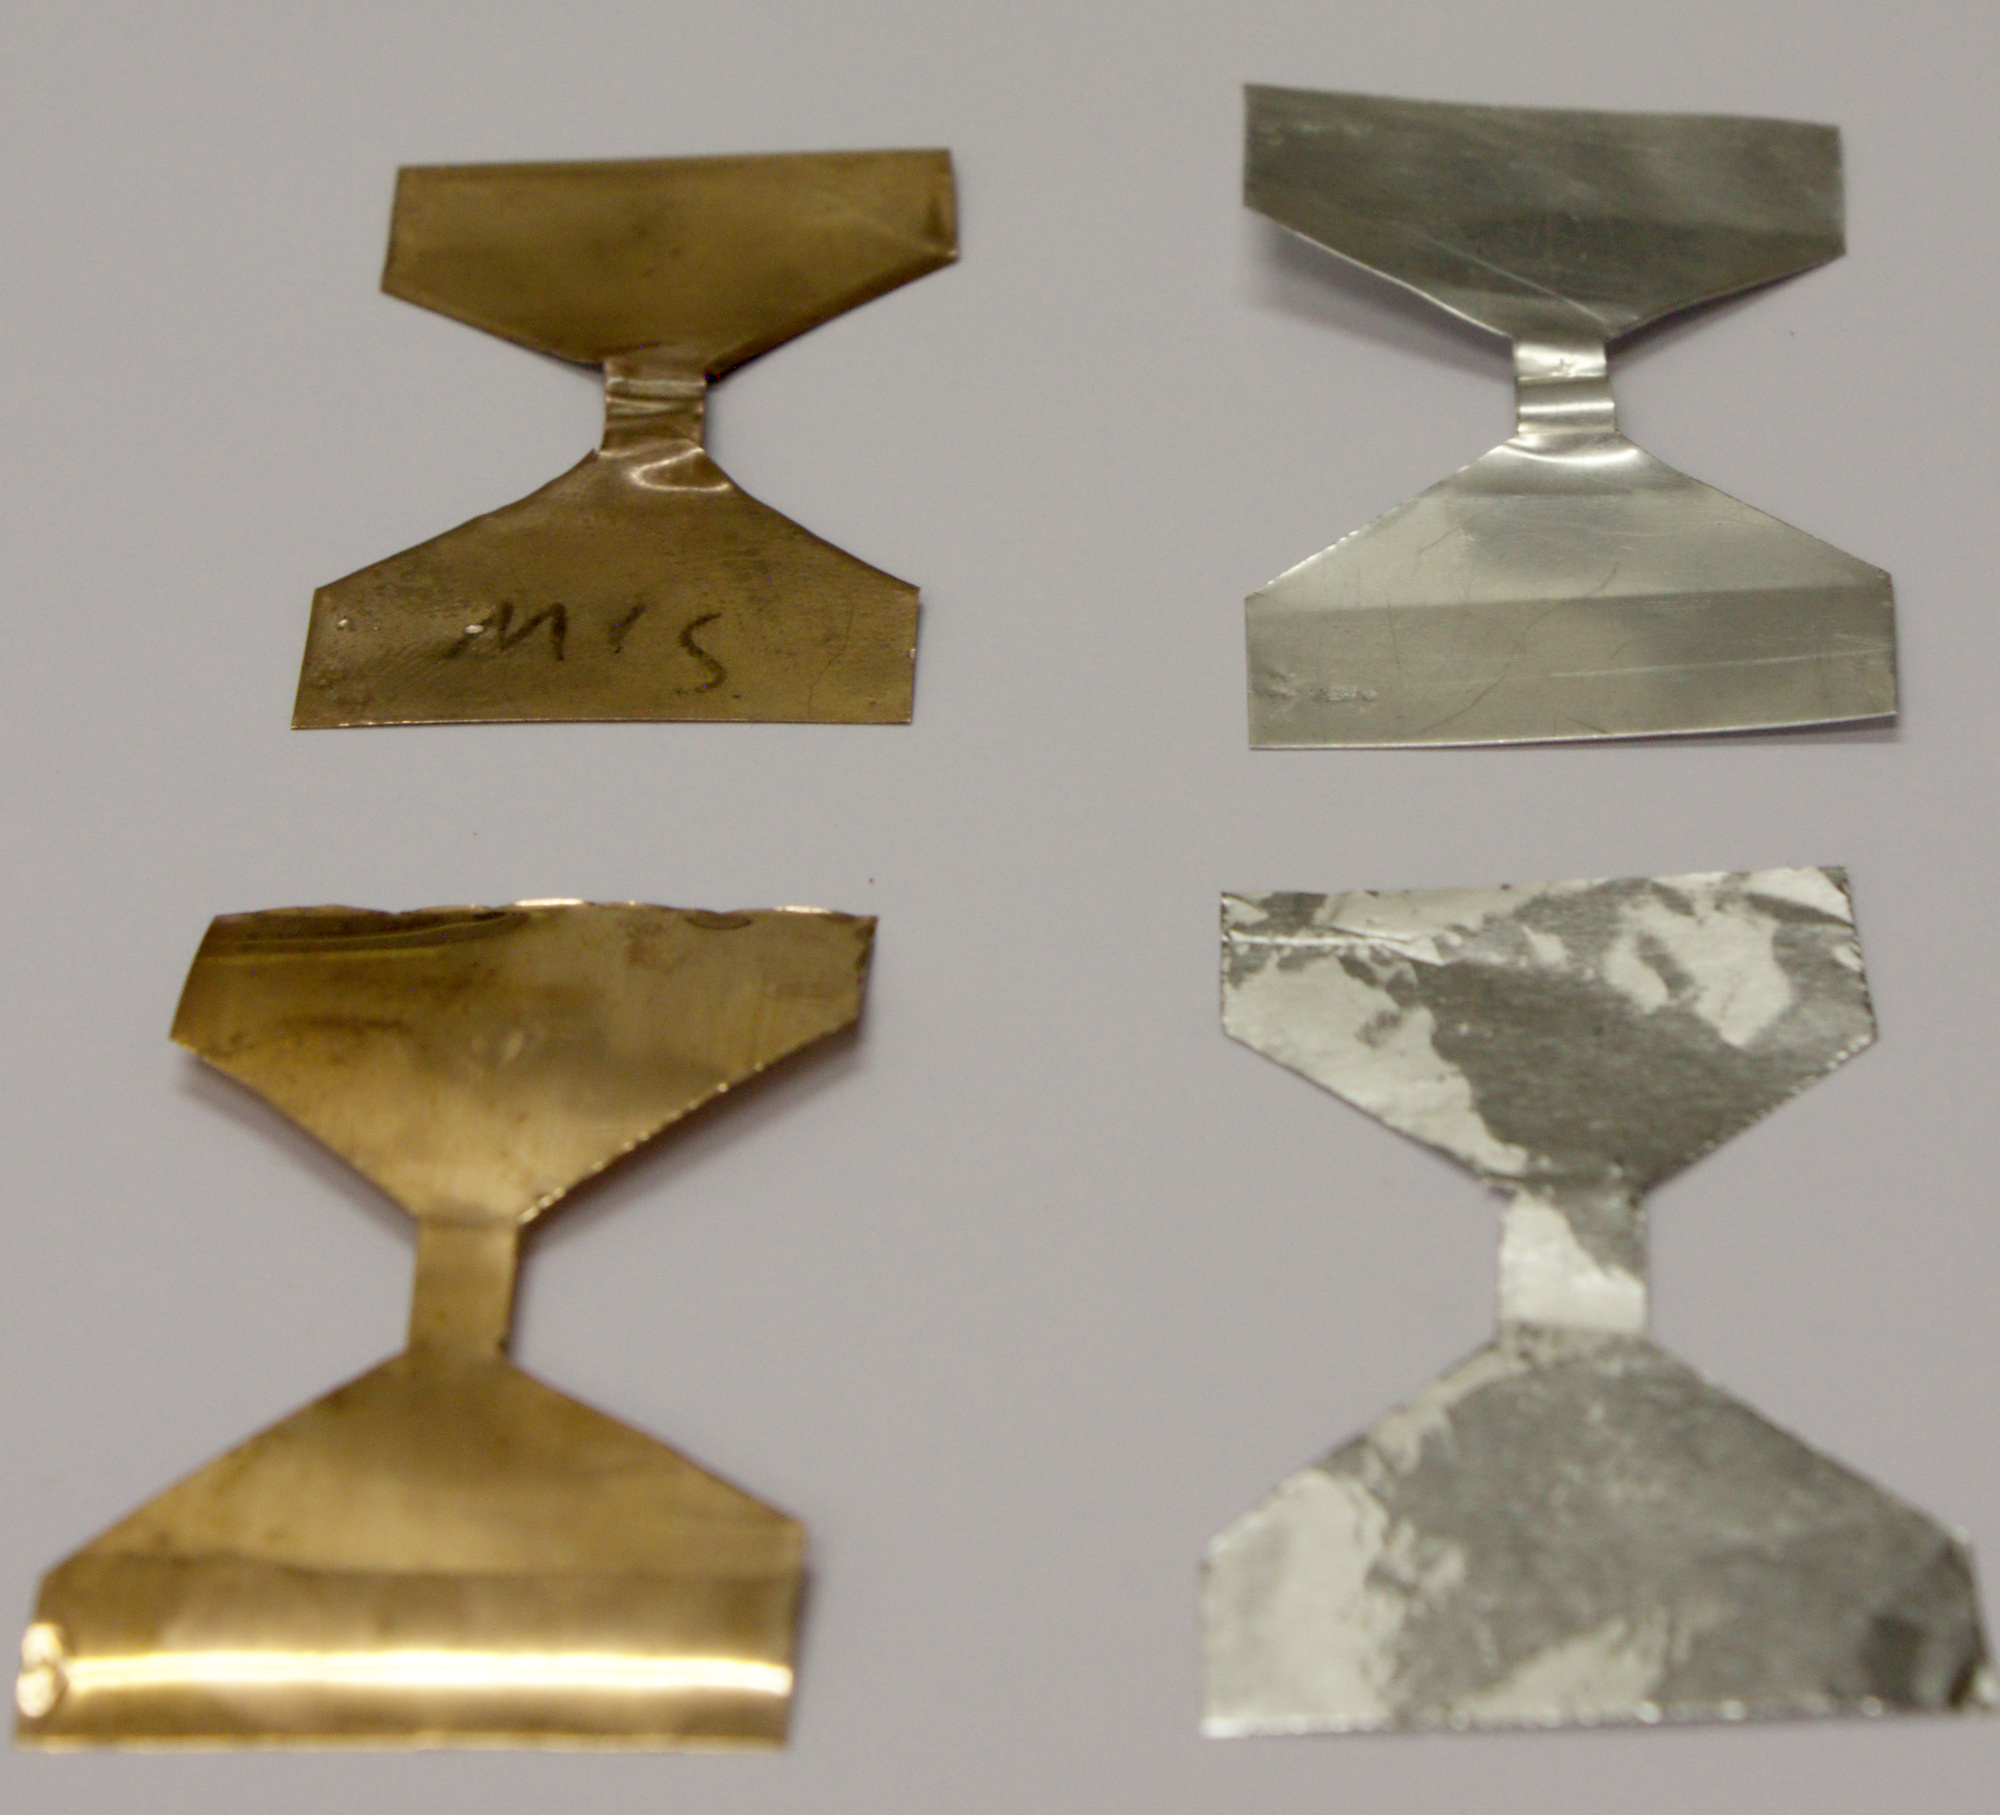
\includegraphics[width=0.4\textwidth]{images/coils}
\quad
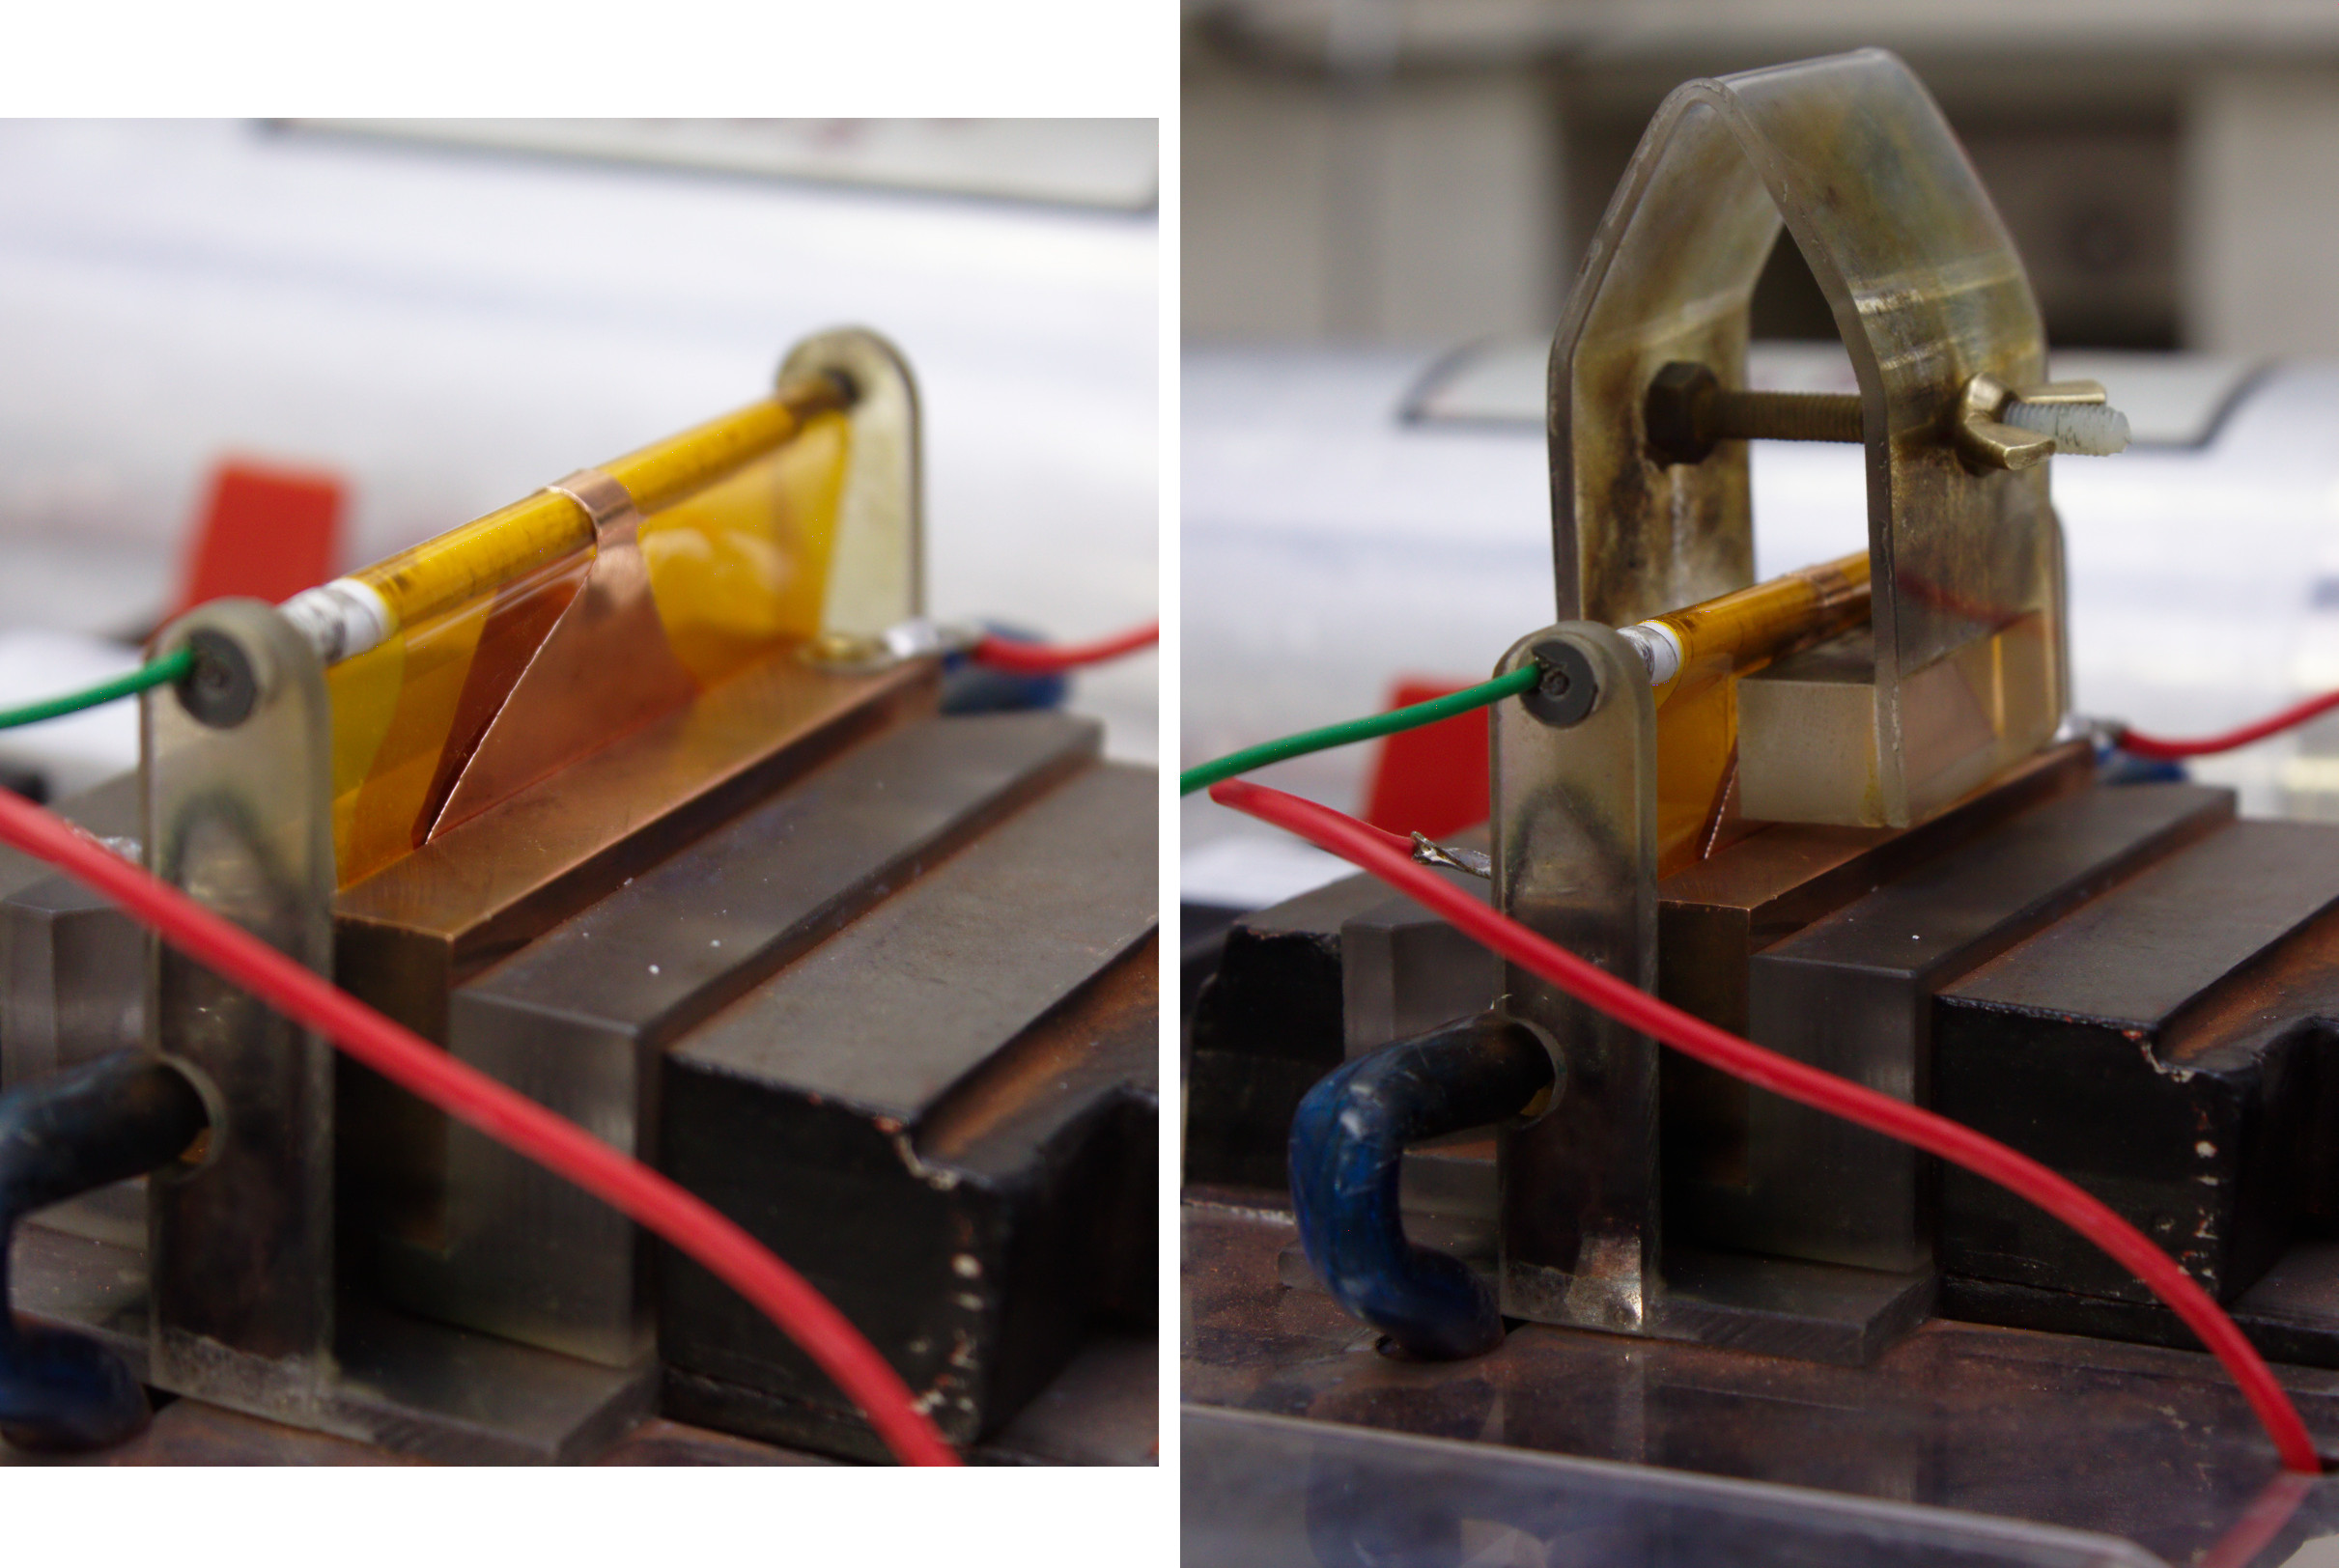
\includegraphics[width=0.5\textwidth]{images/unclampedAndClamped.jpg}
\end{center}
\end{frame}

\subsection{Ons experiment}
\begin{frame}
\begin{columns}
\begin{column}{0.3\textwidth}
	\begin{itemize}
	\item Mobiel apparaat
	\item Kleine schaal
	\item Proof of concept
	\item $\sim2$ tesla
	\item 400\,$\mu$F
	\item 850\,V
	\item 150\,J
	\end{itemize}
\end{column}
\begin{column}{0.7\textwidth}
	\begin{center}
	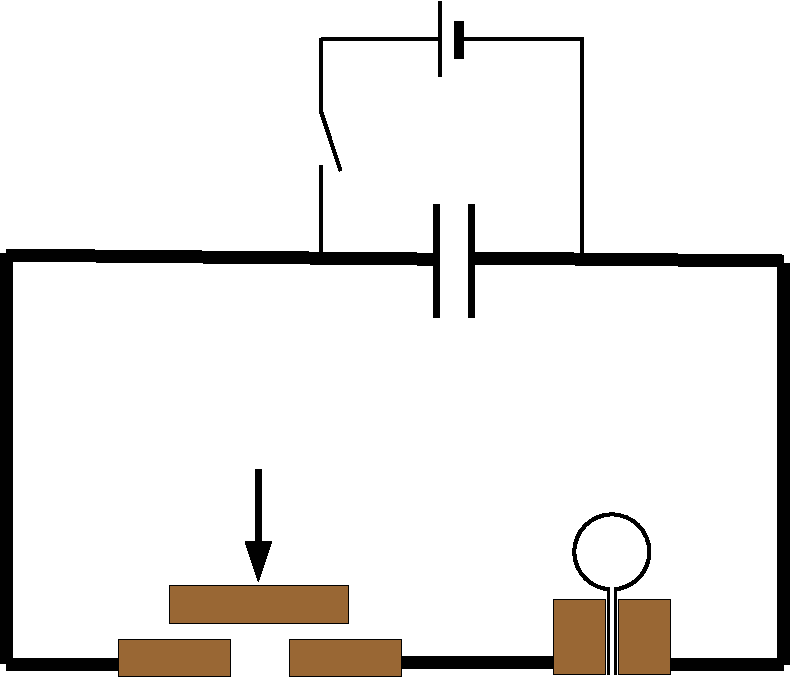
\includegraphics[width=0.5\textwidth]{images/circuit} \\
	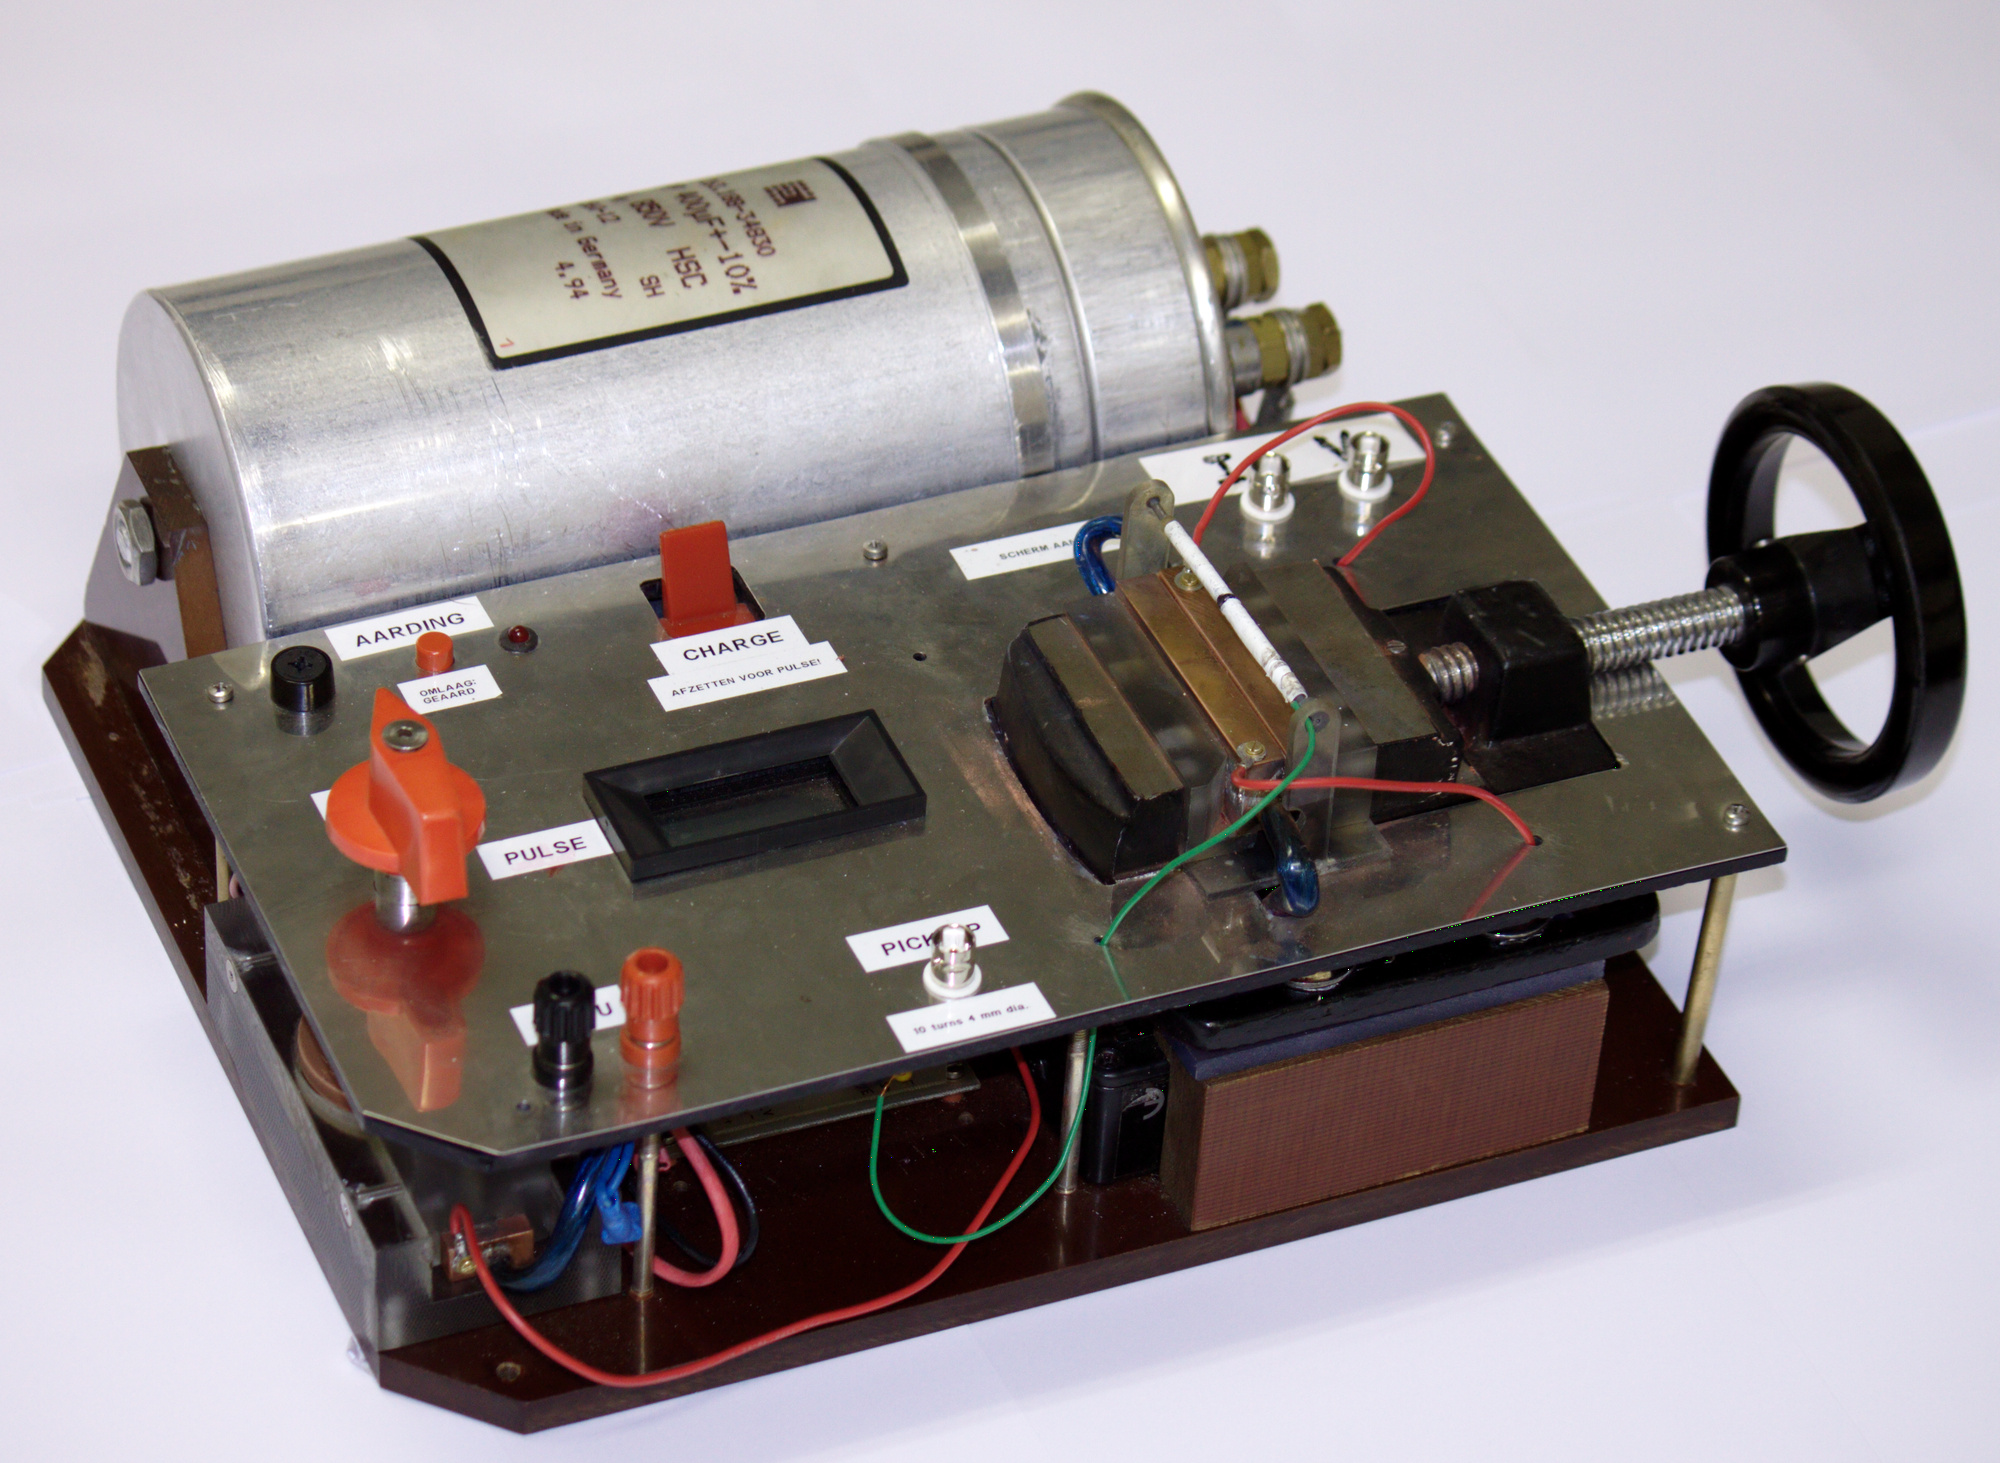
\includegraphics[width=0.8\textwidth]{images/apparatus}
	\end{center}
\end{column}
\end{columns}

\end{frame}

\section{Onze aanpassingen}
\subsection{Wijzigingen}
\begin{frame}
\begin{columns}
\begin{column}{0.5\textwidth}
	\begin{itemize}
	\item Oorspronkelijk
		\begin{itemize}
		\item $\derivs{B}{t}$ pickup-spoel
		\item[$\rightarrow$] Nieuw: 136\,mm$^2$
		\end{itemize}
	\item Onze toevoegingen
		\begin{itemize}
		\item Spanning over spoel
		\item Stroom (door shunt)
		\end{itemize}
	\end{itemize}
\end{column}
\begin{column}{0.5\textwidth}
	\begin{center}
	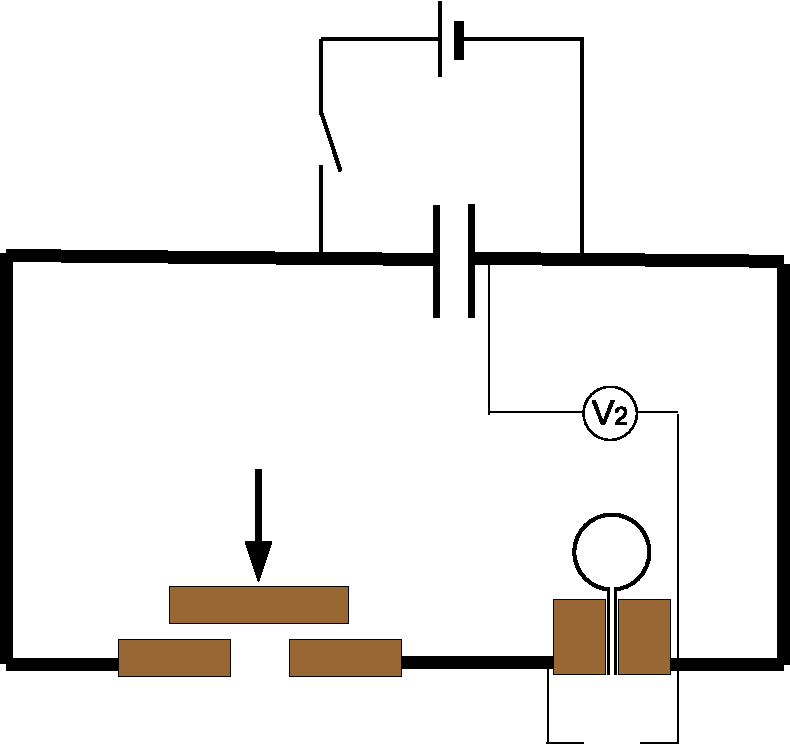
\includegraphics[width=0.9\textwidth]{images/circuit-new}
	\end{center}
\end{column}
\end{columns}
\end{frame}

\subsection{Calibratie}
\begin{frame}
\centering Spanning over shunt $\rightarrow$ Stroom
\begin{itemize}
\item Meting zonder spoel
\item RLC circuit
\item $L$ = parasitare inductantie
\item $C$ gekend
\end{itemize}
\begin{equation*}
I(t) = -V_0 C \frac{\omega}{\sqrt{1-\zeta^2}} e^{-\zeta \omega t} \sin{\omega_d 
t}
\end{equation*}
$$
\omega^2 = \frac{1}{LC} \qquad
\zeta = \frac{R}{2L \omega} \qquad
\omega_d = \omega \sqrt{1-\zeta^2}
$$
\end{frame}

\begin{frame}
\begin{center}
\includeGraph{0.85}{fitI800V}
\end{center}
\end{frame}

\begin{frame}
\centering \scalebox{0.8}{
	\begin{tabular}{c|c|c|c}
	$V_0$ (V)&
		L ($\mu$H)&
				R (m$\Omega$)&
					$\Rshunt$ (m$\Omega$)\\\hline
	71&	0.83 $\pm$ 0.06&	12  $\pm$ 3&	43   $\pm$ 8\\
	100&	0.84 $\pm$ 0.03&	9   $\pm$ 1&	9    $\pm$ 1\\
	200&	0.82 $\pm$ 0.01&	8.3 $\pm$ 0.6&	5.3  $\pm$ 0.3\\
	400&	0.82 $\pm$ 0.01&	7.1 $\pm$ 0.6&	2.0  $\pm$ 0.1\\
	800&	0.82 $\pm$ 0.01&	7.7 $\pm$ 0.7&	1.12 $\pm$ 0.09\\
	\end{tabular}
}
\includeGraph{0.8}{RshuntPlot}
\end{frame}

\begin{frame}
\begin{columns}[c]
\begin{column}[c]{0.5\textwidth}
\includeGraph{0.65}{Ishunt}
\end{column}
\begin{column}[c]{0.5\textwidth}
\begin{center}
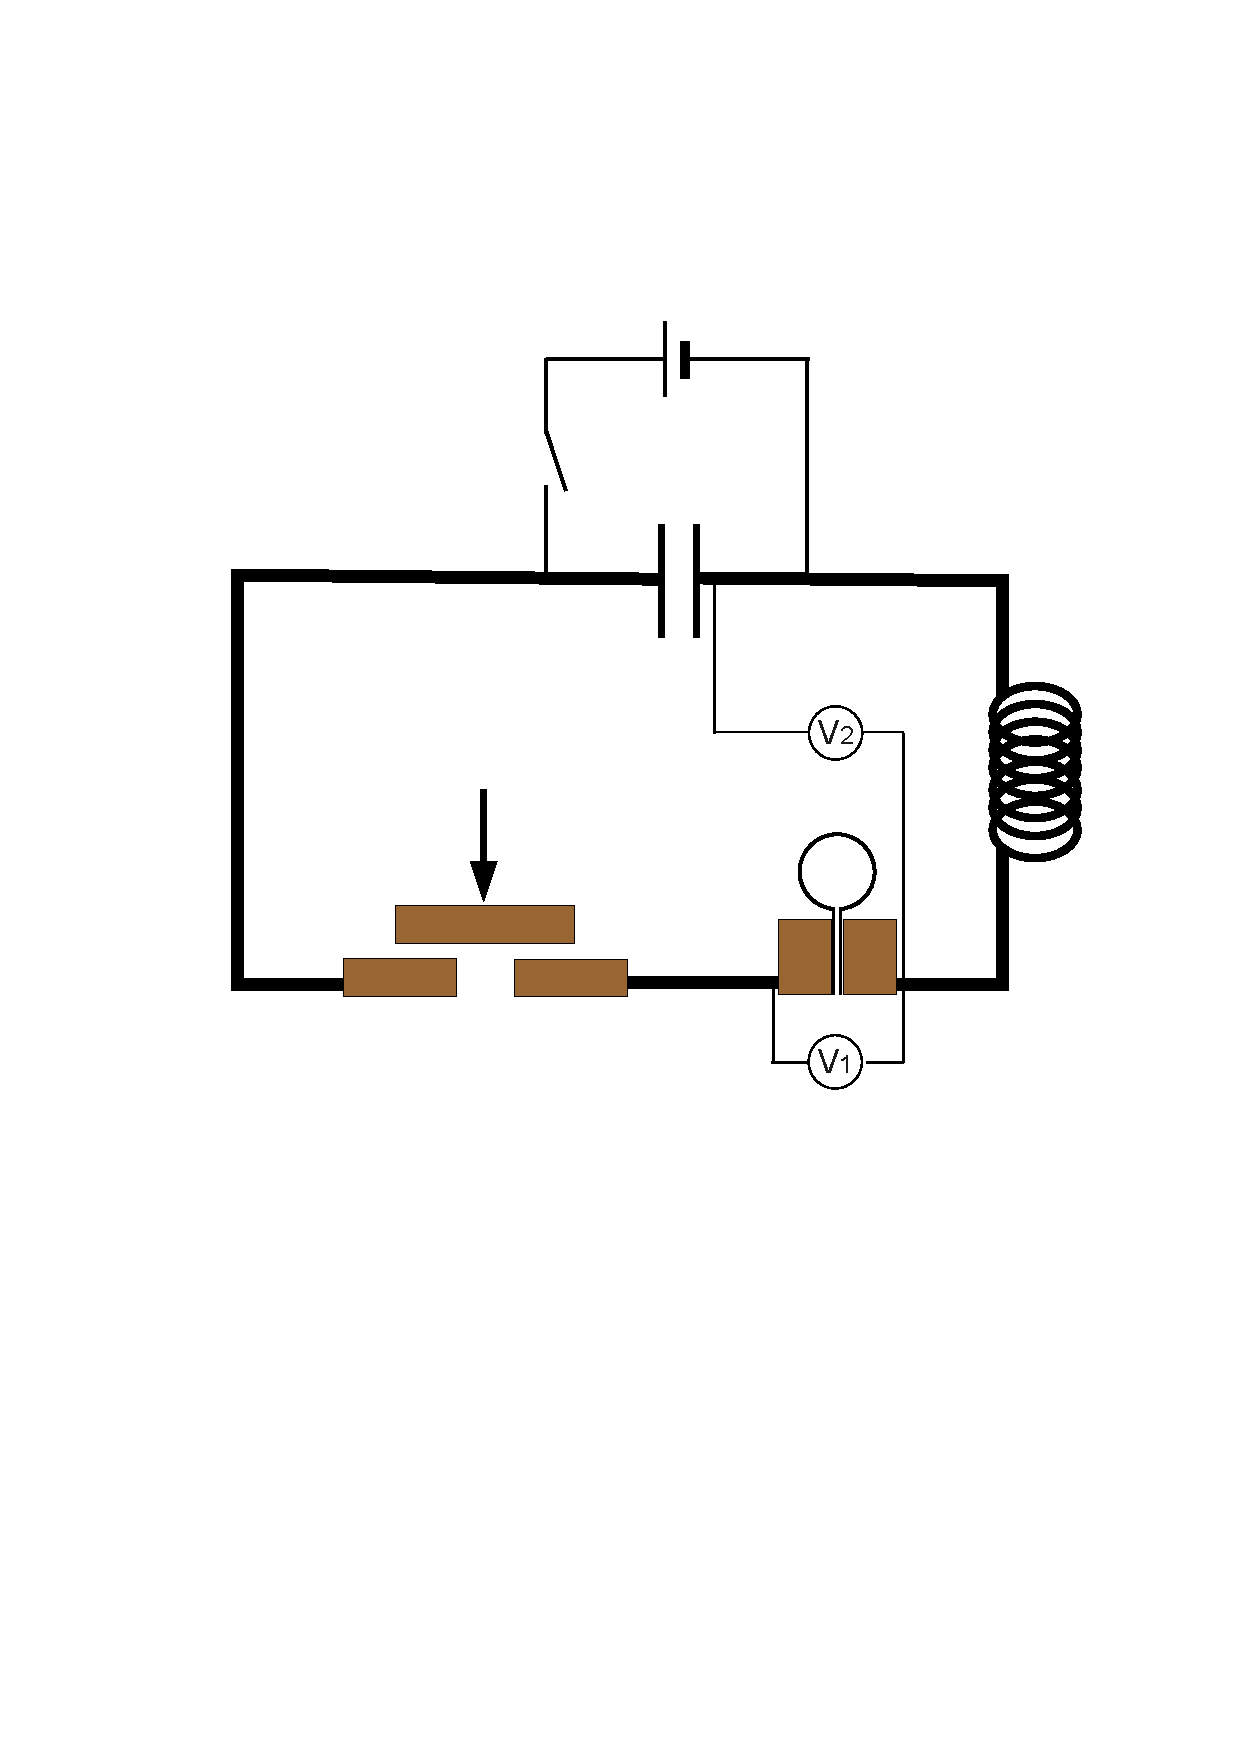
\includegraphics[width=1.0\textwidth]{images/circuit-new-inductance}
\end{center}
\end{column}
\end{columns}
\end{frame}

\section{Resultaten}
\subsection{Piekvelden}
\begin{frame}
\begin{itemize}
\item 127 metingen
\item 28 metingen bij maximale energie
\item 10 piekvelden boven 1\,T
\item Maximaal 2.7\,T
\item Herinner: proof of concept
\end{itemize}
\end{frame}

\begin{frame}
\includeGraph{0.8}{bplot}
\end{frame}

\begin{frame}
Hoger veld
\begin{itemize}
\item Parasitaire $L$ kleiner want energie gedeeld $\rightarrow$ geometrie
\item Grotere $\omega$ $\rightarrow$ $B$ piek v\'o\'or desintegratie 
$\rightarrow$ $L,C\downarrow$
\item Maar meer energie in condensatoren $\rightarrow V \uparrow$
\end{itemize}
\end{frame}



\subsection{Invloed van parameters}
\begin{frame}
\centering Geen invloed van spanning condensator of dikte van spoel meetbaar

\begin{columns}
\begin{column}{0.5\textwidth}
\includeGraph{0.6}{BvasteD}
\end{column}
\begin{column}{0.5\textwidth}
\includeGraph{0.6}{BvasteV}
\end{column}
\end{columns}

\end{frame}

\begin{frame}
\begin{center}
	\includegraphics[width=0.9\textwidth]{images/shortCircuit}
\end{center}
\end{frame}


\subsection{Plasmageleiding}
\begin{frame}

\begin{itemize}
\item Plasmageleiding
\item Karakteristieke knik
\item Dunne materialen zoals aluminium
\end{itemize}

\includeGraph{0.6}{plasma2}
\end{frame}

\begin{frame}
\begin{figure}[c] \includegraphics[width=0.9\textwidth]{images/plasmaArc.jpg}
\end{figure}
\end{frame}

\subsection{Vermogen}
\begin{frame}
\begin{itemize}
\item $P = VI$
\item Enkel kwalitatief!
\end{itemize}
\includeGraph{0.7}{power}
\end{frame}

\section{Conclusie}
\begin{frame}
Conclusie
\begin{itemize}
\item Velden tot 2.7\,T
\item Geen correlatie gevonden met spanning of spoelafmetingen \\
	Wel verwacht (meer metingen)
\item Hoogfrequente signalen meten niet evident
\item Nieuwe fenomenen bestudeerd door extra meetmogelijkheden
\begin{itemize}
	\item Vermogendissipatie in spoel en plasma
	\item Plasmageleiding
	\item Spoelvervorming
\end{itemize}
\end{itemize}
\end{frame}

\section{Dankwoord}
\begin{frame}
\centering Met dank aan Prof. Johan Vanacken \\
\begin{center}
	\includegraphics[width=0.4\textwidth]{images/JvA}
\end{center}
\end{frame}

{
\setbeamercolor{background canvas}{bg=black}
\begin{frame}[plain]
\begin{center}
\mbox{
	\hspace{-3cm}
		\includegraphics[width=\paperwidth]{images/fuckYeah}
	\hspace{-3cm}
}
\end{center}
\end{frame}
}
\end{document}
